% Options for packages loaded elsewhere
\PassOptionsToPackage{unicode}{hyperref}
\PassOptionsToPackage{hyphens}{url}
\PassOptionsToPackage{dvipsnames,svgnames,x11names}{xcolor}
%
\documentclass[
  letterpaper,
  DIV=11,
  numbers=noendperiod]{scrreprt}

\usepackage{amsmath,amssymb}
\usepackage{iftex}
\ifPDFTeX
  \usepackage[T1]{fontenc}
  \usepackage[utf8]{inputenc}
  \usepackage{textcomp} % provide euro and other symbols
\else % if luatex or xetex
  \usepackage{unicode-math}
  \defaultfontfeatures{Scale=MatchLowercase}
  \defaultfontfeatures[\rmfamily]{Ligatures=TeX,Scale=1}
\fi
\usepackage{lmodern}
\ifPDFTeX\else  
    % xetex/luatex font selection
\fi
% Use upquote if available, for straight quotes in verbatim environments
\IfFileExists{upquote.sty}{\usepackage{upquote}}{}
\IfFileExists{microtype.sty}{% use microtype if available
  \usepackage[]{microtype}
  \UseMicrotypeSet[protrusion]{basicmath} % disable protrusion for tt fonts
}{}
\makeatletter
\@ifundefined{KOMAClassName}{% if non-KOMA class
  \IfFileExists{parskip.sty}{%
    \usepackage{parskip}
  }{% else
    \setlength{\parindent}{0pt}
    \setlength{\parskip}{6pt plus 2pt minus 1pt}}
}{% if KOMA class
  \KOMAoptions{parskip=half}}
\makeatother
\usepackage{xcolor}
\setlength{\emergencystretch}{3em} % prevent overfull lines
\setcounter{secnumdepth}{5}
% Make \paragraph and \subparagraph free-standing
\makeatletter
\ifx\paragraph\undefined\else
  \let\oldparagraph\paragraph
  \renewcommand{\paragraph}{
    \@ifstar
      \xxxParagraphStar
      \xxxParagraphNoStar
  }
  \newcommand{\xxxParagraphStar}[1]{\oldparagraph*{#1}\mbox{}}
  \newcommand{\xxxParagraphNoStar}[1]{\oldparagraph{#1}\mbox{}}
\fi
\ifx\subparagraph\undefined\else
  \let\oldsubparagraph\subparagraph
  \renewcommand{\subparagraph}{
    \@ifstar
      \xxxSubParagraphStar
      \xxxSubParagraphNoStar
  }
  \newcommand{\xxxSubParagraphStar}[1]{\oldsubparagraph*{#1}\mbox{}}
  \newcommand{\xxxSubParagraphNoStar}[1]{\oldsubparagraph{#1}\mbox{}}
\fi
\makeatother

\usepackage{color}
\usepackage{fancyvrb}
\newcommand{\VerbBar}{|}
\newcommand{\VERB}{\Verb[commandchars=\\\{\}]}
\DefineVerbatimEnvironment{Highlighting}{Verbatim}{commandchars=\\\{\}}
% Add ',fontsize=\small' for more characters per line
\usepackage{framed}
\definecolor{shadecolor}{RGB}{241,243,245}
\newenvironment{Shaded}{\begin{snugshade}}{\end{snugshade}}
\newcommand{\AlertTok}[1]{\textcolor[rgb]{0.68,0.00,0.00}{#1}}
\newcommand{\AnnotationTok}[1]{\textcolor[rgb]{0.37,0.37,0.37}{#1}}
\newcommand{\AttributeTok}[1]{\textcolor[rgb]{0.40,0.45,0.13}{#1}}
\newcommand{\BaseNTok}[1]{\textcolor[rgb]{0.68,0.00,0.00}{#1}}
\newcommand{\BuiltInTok}[1]{\textcolor[rgb]{0.00,0.23,0.31}{#1}}
\newcommand{\CharTok}[1]{\textcolor[rgb]{0.13,0.47,0.30}{#1}}
\newcommand{\CommentTok}[1]{\textcolor[rgb]{0.37,0.37,0.37}{#1}}
\newcommand{\CommentVarTok}[1]{\textcolor[rgb]{0.37,0.37,0.37}{\textit{#1}}}
\newcommand{\ConstantTok}[1]{\textcolor[rgb]{0.56,0.35,0.01}{#1}}
\newcommand{\ControlFlowTok}[1]{\textcolor[rgb]{0.00,0.23,0.31}{\textbf{#1}}}
\newcommand{\DataTypeTok}[1]{\textcolor[rgb]{0.68,0.00,0.00}{#1}}
\newcommand{\DecValTok}[1]{\textcolor[rgb]{0.68,0.00,0.00}{#1}}
\newcommand{\DocumentationTok}[1]{\textcolor[rgb]{0.37,0.37,0.37}{\textit{#1}}}
\newcommand{\ErrorTok}[1]{\textcolor[rgb]{0.68,0.00,0.00}{#1}}
\newcommand{\ExtensionTok}[1]{\textcolor[rgb]{0.00,0.23,0.31}{#1}}
\newcommand{\FloatTok}[1]{\textcolor[rgb]{0.68,0.00,0.00}{#1}}
\newcommand{\FunctionTok}[1]{\textcolor[rgb]{0.28,0.35,0.67}{#1}}
\newcommand{\ImportTok}[1]{\textcolor[rgb]{0.00,0.46,0.62}{#1}}
\newcommand{\InformationTok}[1]{\textcolor[rgb]{0.37,0.37,0.37}{#1}}
\newcommand{\KeywordTok}[1]{\textcolor[rgb]{0.00,0.23,0.31}{\textbf{#1}}}
\newcommand{\NormalTok}[1]{\textcolor[rgb]{0.00,0.23,0.31}{#1}}
\newcommand{\OperatorTok}[1]{\textcolor[rgb]{0.37,0.37,0.37}{#1}}
\newcommand{\OtherTok}[1]{\textcolor[rgb]{0.00,0.23,0.31}{#1}}
\newcommand{\PreprocessorTok}[1]{\textcolor[rgb]{0.68,0.00,0.00}{#1}}
\newcommand{\RegionMarkerTok}[1]{\textcolor[rgb]{0.00,0.23,0.31}{#1}}
\newcommand{\SpecialCharTok}[1]{\textcolor[rgb]{0.37,0.37,0.37}{#1}}
\newcommand{\SpecialStringTok}[1]{\textcolor[rgb]{0.13,0.47,0.30}{#1}}
\newcommand{\StringTok}[1]{\textcolor[rgb]{0.13,0.47,0.30}{#1}}
\newcommand{\VariableTok}[1]{\textcolor[rgb]{0.07,0.07,0.07}{#1}}
\newcommand{\VerbatimStringTok}[1]{\textcolor[rgb]{0.13,0.47,0.30}{#1}}
\newcommand{\WarningTok}[1]{\textcolor[rgb]{0.37,0.37,0.37}{\textit{#1}}}

\providecommand{\tightlist}{%
  \setlength{\itemsep}{0pt}\setlength{\parskip}{0pt}}\usepackage{longtable,booktabs,array}
\usepackage{calc} % for calculating minipage widths
% Correct order of tables after \paragraph or \subparagraph
\usepackage{etoolbox}
\makeatletter
\patchcmd\longtable{\par}{\if@noskipsec\mbox{}\fi\par}{}{}
\makeatother
% Allow footnotes in longtable head/foot
\IfFileExists{footnotehyper.sty}{\usepackage{footnotehyper}}{\usepackage{footnote}}
\makesavenoteenv{longtable}
\usepackage{graphicx}
\makeatletter
\newsavebox\pandoc@box
\newcommand*\pandocbounded[1]{% scales image to fit in text height/width
  \sbox\pandoc@box{#1}%
  \Gscale@div\@tempa{\textheight}{\dimexpr\ht\pandoc@box+\dp\pandoc@box\relax}%
  \Gscale@div\@tempb{\linewidth}{\wd\pandoc@box}%
  \ifdim\@tempb\p@<\@tempa\p@\let\@tempa\@tempb\fi% select the smaller of both
  \ifdim\@tempa\p@<\p@\scalebox{\@tempa}{\usebox\pandoc@box}%
  \else\usebox{\pandoc@box}%
  \fi%
}
% Set default figure placement to htbp
\def\fps@figure{htbp}
\makeatother
% definitions for citeproc citations
\NewDocumentCommand\citeproctext{}{}
\NewDocumentCommand\citeproc{mm}{%
  \begingroup\def\citeproctext{#2}\cite{#1}\endgroup}
\makeatletter
 % allow citations to break across lines
 \let\@cite@ofmt\@firstofone
 % avoid brackets around text for \cite:
 \def\@biblabel#1{}
 \def\@cite#1#2{{#1\if@tempswa , #2\fi}}
\makeatother
\newlength{\cslhangindent}
\setlength{\cslhangindent}{1.5em}
\newlength{\csllabelwidth}
\setlength{\csllabelwidth}{3em}
\newenvironment{CSLReferences}[2] % #1 hanging-indent, #2 entry-spacing
 {\begin{list}{}{%
  \setlength{\itemindent}{0pt}
  \setlength{\leftmargin}{0pt}
  \setlength{\parsep}{0pt}
  % turn on hanging indent if param 1 is 1
  \ifodd #1
   \setlength{\leftmargin}{\cslhangindent}
   \setlength{\itemindent}{-1\cslhangindent}
  \fi
  % set entry spacing
  \setlength{\itemsep}{#2\baselineskip}}}
 {\end{list}}
\usepackage{calc}
\newcommand{\CSLBlock}[1]{\hfill\break\parbox[t]{\linewidth}{\strut\ignorespaces#1\strut}}
\newcommand{\CSLLeftMargin}[1]{\parbox[t]{\csllabelwidth}{\strut#1\strut}}
\newcommand{\CSLRightInline}[1]{\parbox[t]{\linewidth - \csllabelwidth}{\strut#1\strut}}
\newcommand{\CSLIndent}[1]{\hspace{\cslhangindent}#1}

\KOMAoption{captions}{tableheading}
\makeatletter
\@ifpackageloaded{tcolorbox}{}{\usepackage[skins,breakable]{tcolorbox}}
\@ifpackageloaded{fontawesome5}{}{\usepackage{fontawesome5}}
\definecolor{quarto-callout-color}{HTML}{909090}
\definecolor{quarto-callout-note-color}{HTML}{0758E5}
\definecolor{quarto-callout-important-color}{HTML}{CC1914}
\definecolor{quarto-callout-warning-color}{HTML}{EB9113}
\definecolor{quarto-callout-tip-color}{HTML}{00A047}
\definecolor{quarto-callout-caution-color}{HTML}{FC5300}
\definecolor{quarto-callout-color-frame}{HTML}{acacac}
\definecolor{quarto-callout-note-color-frame}{HTML}{4582ec}
\definecolor{quarto-callout-important-color-frame}{HTML}{d9534f}
\definecolor{quarto-callout-warning-color-frame}{HTML}{f0ad4e}
\definecolor{quarto-callout-tip-color-frame}{HTML}{02b875}
\definecolor{quarto-callout-caution-color-frame}{HTML}{fd7e14}
\makeatother
\makeatletter
\@ifpackageloaded{bookmark}{}{\usepackage{bookmark}}
\makeatother
\makeatletter
\@ifpackageloaded{caption}{}{\usepackage{caption}}
\AtBeginDocument{%
\ifdefined\contentsname
  \renewcommand*\contentsname{Table of contents}
\else
  \newcommand\contentsname{Table of contents}
\fi
\ifdefined\listfigurename
  \renewcommand*\listfigurename{List of Figures}
\else
  \newcommand\listfigurename{List of Figures}
\fi
\ifdefined\listtablename
  \renewcommand*\listtablename{List of Tables}
\else
  \newcommand\listtablename{List of Tables}
\fi
\ifdefined\figurename
  \renewcommand*\figurename{Figure}
\else
  \newcommand\figurename{Figure}
\fi
\ifdefined\tablename
  \renewcommand*\tablename{Table}
\else
  \newcommand\tablename{Table}
\fi
}
\@ifpackageloaded{float}{}{\usepackage{float}}
\floatstyle{ruled}
\@ifundefined{c@chapter}{\newfloat{codelisting}{h}{lop}}{\newfloat{codelisting}{h}{lop}[chapter]}
\floatname{codelisting}{Listing}
\newcommand*\listoflistings{\listof{codelisting}{List of Listings}}
\makeatother
\makeatletter
\makeatother
\makeatletter
\@ifpackageloaded{caption}{}{\usepackage{caption}}
\@ifpackageloaded{subcaption}{}{\usepackage{subcaption}}
\makeatother

\usepackage{bookmark}

\IfFileExists{xurl.sty}{\usepackage{xurl}}{} % add URL line breaks if available
\urlstyle{same} % disable monospaced font for URLs
\hypersetup{
  pdftitle={SF Data Tips and Tricks},
  pdfauthor={OEWD Data and Performance Team},
  colorlinks=true,
  linkcolor={blue},
  filecolor={Maroon},
  citecolor={Blue},
  urlcolor={Blue},
  pdfcreator={LaTeX via pandoc}}


\title{SF Data Tips and Tricks}
\author{OEWD Data and Performance Team}
\date{2024-04-03}

\begin{document}
\maketitle

\renewcommand*\contentsname{Table of contents}
{
\hypersetup{linkcolor=}
\setcounter{tocdepth}{2}
\tableofcontents
}

\bookmarksetup{startatroot}

\chapter*{Introduction}\label{introduction}
\addcontentsline{toc}{chapter}{Introduction}

\markboth{Introduction}{Introduction}

This WIP Quarto `book' is a collection of (mostly R) tips and tricks
relevant to data professionals with the City and County of San
Francisco.

Comments, questions, or suggestions?
\href{https://github.com/SFOEWD/SF-Data-Tips-and-Tricks/issues}{Create
an issue here.}

Edits, additions, or corrections? Open a pull request.

To learn more about Quarto books visit
\url{https://quarto.org/docs/books}.

\begin{center}

\includegraphics[width=2.34375in,height=\textheight,keepaspectratio]{assets/OEWD Circle Logo.png}
\end{center}

\bookmarksetup{startatroot}

\chapter{DataSF}\label{datasf}

Getting data from DataSF is a matter of copying the relevant URL into
one of R's many read functions, e.g.~\texttt{readr::read\_csv},
\texttt{jsonlite::fromJSON}, \texttt{st::st\_read}, etc.

\begin{Shaded}
\begin{Highlighting}[]
\FunctionTok{library}\NormalTok{(readr)}
\FunctionTok{library}\NormalTok{(sf)}
\end{Highlighting}
\end{Shaded}

\begin{verbatim}
Linking to GEOS 3.9.1, GDAL 3.4.3, PROJ 7.2.1; sf_use_s2() is TRUE
\end{verbatim}

\begin{Shaded}
\begin{Highlighting}[]
\NormalTok{reg\_businesses }\OtherTok{\textless{}{-}} \FunctionTok{read\_csv}\NormalTok{(}\StringTok{"https://data.sfgov.org/resource/g8m3{-}pdis.csv"}\NormalTok{)}
\end{Highlighting}
\end{Shaded}

\begin{verbatim}
Rows: 1000 Columns: 37
\end{verbatim}

\begin{verbatim}
-- Column specification --------------------------------------------------------
Delimiter: ","
chr  (22): uniqueid, ttxid, certificate_number, ownership_name, dba_name, fu...
dbl   (7): business_zip, supervisor_district, :@computed_region_6qbp_sg9q, :...
lgl   (2): parking_tax, transient_occupancy_tax
dttm  (6): dba_start_date, dba_end_date, location_start_date, location_end_d...

i Use `spec()` to retrieve the full column specification for this data.
i Specify the column types or set `show_col_types = FALSE` to quiet this message.
\end{verbatim}

\begin{tcolorbox}[enhanced jigsaw, breakable, coltitle=black, opacitybacktitle=0.6, opacityback=0, leftrule=.75mm, colbacktitle=quarto-callout-warning-color!10!white, toprule=.15mm, colframe=quarto-callout-warning-color-frame, colback=white, left=2mm, bottomrule=.15mm, rightrule=.15mm, bottomtitle=1mm, toptitle=1mm, title=\textcolor{quarto-callout-warning-color}{\faExclamationTriangle}\hspace{0.5em}{Warning}, titlerule=0mm, arc=.35mm]

Behind the scenes there is a limit parameter that defaults to 1000,
\emph{even if the `All data' radio button is selected.} To retrieve all
the data, either read the same URL with the RSocrata package:\\

\begin{Shaded}
\begin{Highlighting}[]
\NormalTok{reg\_businesses }\OtherTok{\textless{}{-}}\NormalTok{ RSocrata}\SpecialCharTok{::}\FunctionTok{read.socrata}\NormalTok{(}\StringTok{"https://data.sfgov.org/resource/g8m3{-}pdis.csv"}\NormalTok{)}
\end{Highlighting}
\end{Shaded}

Or append \texttt{?\$limit=9999999} to the end of the URL:

\begin{Shaded}
\begin{Highlighting}[]
\NormalTok{reg\_businesses }\OtherTok{\textless{}{-}} \FunctionTok{read\_csv}\NormalTok{(}\StringTok{"https://data.sfgov.org/resource/g8m3{-}pdis.csv?$limit=9999999"}\NormalTok{)}
\end{Highlighting}
\end{Shaded}

\end{tcolorbox}

Read in a `spatial' object with \texttt{st\_read} and the URL with the
geojson file extension:

\begin{Shaded}
\begin{Highlighting}[]
\NormalTok{sup\_dists }\OtherTok{\textless{}{-}} \FunctionTok{st\_read}\NormalTok{(}\StringTok{"https://data.sfgov.org/api/geospatial/f2zs{-}jevy?accessType=DOWNLOAD\&method=export\&format=GeoJSON"}\NormalTok{)}
\end{Highlighting}
\end{Shaded}

\begin{verbatim}
Reading layer `OGRGeoJSON' from data source 
  `https://data.sfgov.org/api/geospatial/f2zs-jevy?accessType=DOWNLOAD&method=export&format=GeoJSON' 
  using driver `GeoJSON'
Simple feature collection with 11 features and 7 fields
Geometry type: MULTIPOLYGON
Dimension:     XY
Bounding box:  xmin: -123.1738 ymin: 37.63983 xmax: -122.3279 ymax: 37.8632
Geodetic CRS:  WGS 84
\end{verbatim}

\bookmarksetup{startatroot}

\chapter{Excel Stuff}\label{excel-stuff}

\href{https://readxl.tidyverse.org/}{\{readxl\}} is the best package to
\emph{read} excel (xlsx) files.

\begin{Shaded}
\begin{Highlighting}[]
\FunctionTok{library}\NormalTok{(readxl)}
\NormalTok{df }\OtherTok{\textless{}{-}} \FunctionTok{read\_xlsx}\NormalTok{(}\StringTok{"path\_to\_xlsx"}\NormalTok{)}
\end{Highlighting}
\end{Shaded}

\href{https://docs.ropensci.org/writexl/}{\{writexl\}} is the best
package to \emph{write} excel (xlsx) files.

\begin{Shaded}
\begin{Highlighting}[]
\FunctionTok{library}\NormalTok{(writexl)}
\FunctionTok{write\_xlsx}\NormalTok{(mtcars, }\StringTok{"car\_data.xlsx"}\NormalTok{)}
\end{Highlighting}
\end{Shaded}

\section{Miscellaneous Tips and
Tricks}\label{miscellaneous-tips-and-tricks}

You can also pass a named list of data frames to \texttt{write\_xlsx},
and it will write each data frame to a separate sheet in the workbook.

\begin{Shaded}
\begin{Highlighting}[]
\NormalTok{l }\OtherTok{\textless{}{-}} \FunctionTok{list}\NormalTok{(}
  \StringTok{"Car data"} \OtherTok{=}\NormalTok{ mtcars,}
  \StringTok{"Flower data"} \OtherTok{=}\NormalTok{ iris}
\NormalTok{)}

\FunctionTok{write\_xlsx}\NormalTok{(l, }\StringTok{"my\_data.xlsx"}\NormalTok{)}
\end{Highlighting}
\end{Shaded}

With the \texttt{\{purrr\}} package you can look through a directory of
identically structured spreadsheets and bind them together:

\begin{Shaded}
\begin{Highlighting}[]
\FunctionTok{library}\NormalTok{(purrr)}
\FunctionTok{dir}\NormalTok{(}\StringTok{"path\_to\_directory"}\NormalTok{, }\AttributeTok{full.names =} \ConstantTok{TRUE}\NormalTok{) }\SpecialCharTok{\%\textgreater{}\%} 
  \FunctionTok{map\_dfr}\NormalTok{(\textbackslash{}(file) }\FunctionTok{read\_csv}\NormalTok{(file)) }\CommentTok{\# or map(\textbackslash{}(file) read\_csv(file)) \%\textgreater{}\% list\_rbind()}
\end{Highlighting}
\end{Shaded}

With the \href{https://github.com/daranzolin/kapow}{\texttt{\{kapow\}}
package} package you can loop through each sheet in an xlsx workbook and
assign the table to its sheet name in your global environment:

\begin{Shaded}
\begin{Highlighting}[]
\FunctionTok{library}\NormalTok{(readxl)}
\FunctionTok{library}\NormalTok{(purrr)}
\FunctionTok{library}\NormalTok{(kapow) }\CommentTok{\# remotes::install\_github("daranzolin/kapow)}

\NormalTok{xlsx\_path }\OtherTok{\textless{}{-}} \StringTok{"path\_to\_xlsx"}
\NormalTok{sheet\_names }\OtherTok{\textless{}{-}} \FunctionTok{excel\_sheets}\NormalTok{(xlsx\_path)}
\NormalTok{sheet\_names }\SpecialCharTok{\%\textgreater{}\%} 
  \FunctionTok{map}\NormalTok{(\textbackslash{}(sheet) }\FunctionTok{read\_excel}\NormalTok{(xlsx\_path, }\AttributeTok{sheet =}\NormalTok{ sheet)) }\SpecialCharTok{\%\textgreater{}\%} 
  \FunctionTok{set\_names}\NormalTok{(sheet\_names) }\SpecialCharTok{\%\textgreater{}\%} 
  \FunctionTok{kapow}\NormalTok{()}
\end{Highlighting}
\end{Shaded}

To apply special formatting to an Excel workbook in R you can use the
\href{https://github.com/ycphs/openxlsx}{\{openxlsx\} package.} Here's
an example of how OEWD writes to xlsx:

\begin{Shaded}
\begin{Highlighting}[]
\FunctionTok{library}\NormalTok{(openxlsx)}
\NormalTok{write\_oewd\_xlsx }\OtherTok{\textless{}{-}} \ControlFlowTok{function}\NormalTok{(data, sheet\_name, file, }\AttributeTok{dateFormat =} \StringTok{"yyyy/mm/dd"}\NormalTok{, }\AttributeTok{overwrite =} \ConstantTok{FALSE}\NormalTok{) \{}
\NormalTok{  wb }\OtherTok{\textless{}{-}} \FunctionTok{createWorkbook}\NormalTok{()}
  \FunctionTok{addWorksheet}\NormalTok{(wb, sheet\_name)}
\NormalTok{  style }\OtherTok{\textless{}{-}} \FunctionTok{createStyle}\NormalTok{(}\AttributeTok{halign =} \StringTok{"LEFT"}\NormalTok{, }\AttributeTok{valign =} \StringTok{"CENTER"}\NormalTok{)}
  \FunctionTok{setColWidths}\NormalTok{(wb, }\AttributeTok{sheet =} \DecValTok{1}\NormalTok{, }\AttributeTok{cols =} \DecValTok{1}\SpecialCharTok{:}\FunctionTok{ncol}\NormalTok{(data), }\AttributeTok{widths =} \StringTok{"auto"}\NormalTok{)}
  \FunctionTok{addStyle}\NormalTok{(wb, }\DecValTok{1}\NormalTok{,}
           \AttributeTok{cols =} \DecValTok{1}\SpecialCharTok{:}\NormalTok{(}\FunctionTok{ncol}\NormalTok{(data) }\SpecialCharTok{+} \DecValTok{1}\NormalTok{),}
           \AttributeTok{rows =} \DecValTok{1}\SpecialCharTok{:}\NormalTok{(}\FunctionTok{nrow}\NormalTok{(data) }\SpecialCharTok{+} \DecValTok{1}\NormalTok{),}
           \AttributeTok{style =}\NormalTok{ style,}
           \AttributeTok{gridExpand =} \ConstantTok{TRUE}\NormalTok{)}
\NormalTok{  headerStyle }\OtherTok{\textless{}{-}} \FunctionTok{createStyle}\NormalTok{(}
    \AttributeTok{halign =} \StringTok{"LEFT"}\NormalTok{,}
    \AttributeTok{textDecoration =} \StringTok{"Bold"}
\NormalTok{  )}
  \FunctionTok{writeData}\NormalTok{(wb, }\DecValTok{1}\NormalTok{, data, }\AttributeTok{headerStyle =}\NormalTok{ headerStyle)}
  \FunctionTok{options}\NormalTok{(}\StringTok{"openxlsx.dateFormat"} \OtherTok{=}\NormalTok{ dateFormat)}
  \FunctionTok{saveWorkbook}\NormalTok{(wb, file, }\AttributeTok{overwrite =}\NormalTok{ overwrite)}
\NormalTok{\}}

\FunctionTok{write\_oewd\_xlsx}\NormalTok{(mtcars, }\StringTok{"Car data"}\NormalTok{, }\StringTok{"car\_data.xlsx"}\NormalTok{)}
\end{Highlighting}
\end{Shaded}

\bookmarksetup{startatroot}

\chapter{Sharepoint}\label{sharepoint}

Sharepoint is part of many data pipelines, and the easiest way to
interact with Sharepoint from R is through the
\href{https://github.com/Azure/Microsoft365R}{\{Microsoft365R\}
package.} This package has been vetted by the Department of Technology
(DT) and authentication should be straight-forward after calling one of
the initial functions.

\begin{Shaded}
\begin{Highlighting}[]
\FunctionTok{library}\NormalTok{(Microsoft365R)}

\NormalTok{wp }\OtherTok{\textless{}{-}} \FunctionTok{get\_sharepoint\_site}\NormalTok{(}\StringTok{"Workforce Programs"}\NormalTok{)}
\NormalTok{wp\_docs }\OtherTok{\textless{}{-}}\NormalTok{ wp}\SpecialCharTok{$}\FunctionTok{get\_drive}\NormalTok{(}\StringTok{"Documents"}\NormalTok{)}

\NormalTok{wp\_docs}\SpecialCharTok{$}\FunctionTok{list\_files}\NormalTok{()}

\NormalTok{wp\_docs}\SpecialCharTok{$}\FunctionTok{download\_file}\NormalTok{(}\StringTok{"path\_to\_file.xlsx"}\NormalTok{)}
\end{Highlighting}
\end{Shaded}

It is helpful to wrap common read/write operations into more usable
functions:

\begin{Shaded}
\begin{Highlighting}[]
\NormalTok{connect\_to\_sharepoint\_site\_docs }\OtherTok{\textless{}{-}} \ControlFlowTok{function}\NormalTok{(sp\_site) \{}
\NormalTok{  sp\_site }\OtherTok{\textless{}{-}}\NormalTok{ Microsoft365R}\SpecialCharTok{::}\FunctionTok{get\_sharepoint\_site}\NormalTok{(sp\_site)}
\NormalTok{  sp\_site\_doc }\OtherTok{\textless{}{-}}\NormalTok{ sp\_site}\SpecialCharTok{$}\FunctionTok{get\_drive}\NormalTok{(}\StringTok{"Documents"}\NormalTok{)}
  \FunctionTok{return}\NormalTok{(sp\_site\_doc)}
\NormalTok{\}}

\NormalTok{connect\_to\_wp\_docs }\OtherTok{\textless{}{-}} \ControlFlowTok{function}\NormalTok{() }\FunctionTok{connect\_to\_sharepoint\_site\_docs}\NormalTok{(}\StringTok{"Workforce Programs"}\NormalTok{)}

\NormalTok{download\_from\_wp }\OtherTok{\textless{}{-}} \ControlFlowTok{function}\NormalTok{(sp\_file, destination) \{}
\NormalTok{  docs }\OtherTok{\textless{}{-}} \FunctionTok{connect\_to\_wp\_docs}\NormalTok{()}
\NormalTok{  docs}\SpecialCharTok{$}\FunctionTok{download\_file}\NormalTok{(sp\_file, }\AttributeTok{dest =}\NormalTok{ destination)}
\NormalTok{  cli}\SpecialCharTok{::}\FunctionTok{cli\_alert\_success}\NormalTok{(glue}\SpecialCharTok{::}\FunctionTok{glue}\NormalTok{(}\StringTok{"\{sp\_file\} downloaded."}\NormalTok{))}
\NormalTok{\}}

\NormalTok{upload\_to\_wp }\OtherTok{\textless{}{-}} \ControlFlowTok{function}\NormalTok{(file, sp\_destination) \{}
\NormalTok{  docs }\OtherTok{\textless{}{-}} \FunctionTok{connect\_to\_wp\_docs}\NormalTok{()}
\NormalTok{  docs}\SpecialCharTok{$}\FunctionTok{upload\_file}\NormalTok{(}
\NormalTok{    file,}
\NormalTok{    sp\_location}
\NormalTok{  )}
\NormalTok{  cli}\SpecialCharTok{::}\FunctionTok{cli\_alert\_success}\NormalTok{(glue}\SpecialCharTok{::}\FunctionTok{glue}\NormalTok{(}\StringTok{"\{file\} uploaded."}\NormalTok{))}
\NormalTok{\}}

\NormalTok{read\_wp }\OtherTok{\textless{}{-}} \ControlFlowTok{function}\NormalTok{(path) \{}
\NormalTok{  tmp }\OtherTok{\textless{}{-}} \FunctionTok{tempfile}\NormalTok{(}\AttributeTok{fileext =} \StringTok{"xlsx"}\NormalTok{)}
  \FunctionTok{download\_from\_wp}\NormalTok{(}
    \AttributeTok{sp\_file =} \FunctionTok{glue}\NormalTok{(}\StringTok{"\{path\}.xlsx"}\NormalTok{),}
    \AttributeTok{destination =}\NormalTok{ tmp}
\NormalTok{  )}
\NormalTok{  out }\OtherTok{\textless{}{-}}\NormalTok{ readxl}\SpecialCharTok{::}\FunctionTok{read\_excel}\NormalTok{(tmp, }\AttributeTok{.name\_repair =}\NormalTok{ janitor}\SpecialCharTok{::}\NormalTok{make\_clean\_names)}
  \FunctionTok{return}\NormalTok{(out)}
\NormalTok{\}}
\end{Highlighting}
\end{Shaded}

\bookmarksetup{startatroot}

\chapter{Spatial Stuff}\label{spatial-stuff}

The most essential packages for doing GIS work (with ESRI products) are:

\begin{itemize}
\tightlist
\item
  sf
\item
  mapview
\item
  arcgis
\item
  arcgisutils
\item
  arcgislayers
\item
  arcgisbinding
\item
  tidycensus
\end{itemize}

Honorable mention:

\begin{itemize}
\tightlist
\item
  tmap
\item
  terra
\item
  leaflet
\end{itemize}

\begin{Shaded}
\begin{Highlighting}[]
\FunctionTok{library}\NormalTok{(sf)}
\end{Highlighting}
\end{Shaded}

\begin{verbatim}
Linking to GEOS 3.9.1, GDAL 3.4.3, PROJ 7.2.1; sf_use_s2() is TRUE
\end{verbatim}

\begin{Shaded}
\begin{Highlighting}[]
\FunctionTok{library}\NormalTok{(mapview)}
\FunctionTok{library}\NormalTok{(arcgis)}
\end{Highlighting}
\end{Shaded}

\begin{verbatim}
Attaching core arcgis packages:
\end{verbatim}

\begin{verbatim}
> arcgisutils v0.1.1.9000
> arcgislayers v0.1.0
\end{verbatim}

\begin{Shaded}
\begin{Highlighting}[]
\FunctionTok{library}\NormalTok{(tidyverse)}
\end{Highlighting}
\end{Shaded}

\begin{verbatim}
-- Attaching packages --------------------------------------- tidyverse 1.3.2 --
v ggplot2 3.5.1     v purrr   1.0.2
v tibble  3.2.1     v dplyr   1.1.0
v tidyr   1.2.1     v stringr 1.5.0
v readr   2.1.3     v forcats 0.5.2
-- Conflicts ------------------------------------------ tidyverse_conflicts() --
x purrr::%||%()    masks arcgisutils::%||%()
x purrr::compact() masks arcgisutils::compact()
x dplyr::filter()  masks stats::filter()
x dplyr::lag()     masks stats::lag()
\end{verbatim}

\section{ArcGIS REST API}\label{arcgis-rest-api}

The \href{https://github.com/R-ArcGIS/arcgislayers}{\{arcgislayers\}
package} allows users to read and write data from and to the ArcGIS REST
API.

\subsection{Reading Layers}\label{reading-layers}

\begin{Shaded}
\begin{Highlighting}[]
\NormalTok{sf\_libraries\_url }\OtherTok{\textless{}{-}} \StringTok{"https://services.arcgis.com/Zs2aNLFN00jrS4gG/arcgis/rest/services/SF\_Libraries/FeatureServer"}
\CommentTok{\# arc\_open can read a FeatureServer or a FeatureLayer directly}
\NormalTok{(sf\_libraries\_fs }\OtherTok{\textless{}{-}} \FunctionTok{arc\_open}\NormalTok{(sf\_libraries\_url))}
\end{Highlighting}
\end{Shaded}

\begin{verbatim}
<FeatureServer <2 layers, 0 tables>>
CRS: 3857
Capabilities: Query
  0: Libraries (esriGeometryPoint)
  1: Libraries with Air Conditioning (esriGeometryPoint)
\end{verbatim}

\begin{Shaded}
\begin{Highlighting}[]
\NormalTok{(sf\_libraries\_lyr }\OtherTok{\textless{}{-}} \FunctionTok{get\_layer}\NormalTok{(sf\_libraries\_fs, }\AttributeTok{name =} \StringTok{"Libraries"}\NormalTok{))}
\end{Highlighting}
\end{Shaded}

\begin{verbatim}
<FeatureLayer>
Name: Libraries
Geometry Type: esriGeometryPoint
CRS: 3857
Capabilities: Query
\end{verbatim}

\begin{Shaded}
\begin{Highlighting}[]
\NormalTok{sf\_libraries }\OtherTok{\textless{}{-}} \FunctionTok{arc\_select}\NormalTok{(sf\_libraries\_lyr)}
\end{Highlighting}
\end{Shaded}

\begin{verbatim}
Registered S3 method overwritten by 'jsonify':
  method     from    
  print.json jsonlite
\end{verbatim}

\begin{Shaded}
\begin{Highlighting}[]
\FunctionTok{glimpse}\NormalTok{(sf\_libraries)}
\end{Highlighting}
\end{Shaded}

\begin{verbatim}
Rows: 33
Columns: 23
$ objectid         <int> 1, 2, 3, 4, 5, 6, 7, 8, 9, 10, 11, 12, 13, 14, 15, 16~
$ gross_sq_f       <chr> "8500", "6465", "6096", "8536", "7633", "6100", "8000~
$ block_lot        <chr> "8708110", "3564095", "6539034", "2919031", "0469001"~
$ zip_code         <chr> "94158", "94114", "94114", "94127", "94123", "94112",~
$ facility_i       <chr> "1113", "648", "1184", "1853", "1053", "896", "1858",~
$ city             <chr> "San Francisco", "San Francisco", "San Francisco", "S~
$ latitude         <chr> "37.775369728", "37.76406037", "37.750228042", "37.74~
$ department       <chr> "Public Library", "Public Library", "Public Library",~
$ longitude        <chr> "-122.393097384", "-122.431881717", "-122.435090242",~
$ dept_id          <chr> "48", "48", "48", "48", "48", "48", "48", "48", "48",~
$ common_nam       <chr> "Mission Bay Library", "Eureka Valley Branch Library/~
$ address          <chr> "960 04th St", "1 Jose Sarria Ct", "451 Jersey St", "~
$ supervisor       <chr> "6", "8", "8", "7", "2", "7", "5", "6", "10", "8", "9~
$ city_tenan       <chr> " ", " ", " ", " ", " ", " ", " ", " ", " ", " ", " "~
$ owned_leas       <chr> "Own", "Own", "Own", "Own", "Own", "Own", "Own", "Own~
$ globalid         <chr> "755632fc-18d9-4c0e-b65d-ec53d18a132b", "195a2a2b-302~
$ created_user     <chr> "nancy.milholland_sfdem", "nancy.milholland_sfdem", "~
$ created_date     <dttm> 2019-06-07 21:44:34, 2019-06-07 21:44:34, 2019-06-07~
$ last_edited_user <chr> "nancy.milholland_sfdem", "nancy.milholland_sfdem", "~
$ last_edited_date <dttm> 2019-06-07 21:44:34, 2019-06-07 21:44:34, 2019-06-07~
$ eas_id           <lgl> NA, NA, NA, NA, NA, NA, NA, NA, NA, NA, NA, NA, NA, N~
$ air_conditioning <chr> "Yes", "No", "No", "No", "No", "No", "No", "No", "Sec~
$ geometry         <POINT [m]> POINT (-13624737 4547742), POINT (-13629055 454~
\end{verbatim}

\begin{Shaded}
\begin{Highlighting}[]
\CommentTok{\# You can also specify which columns to select, e.g.:}
\CommentTok{\# arc\_select(}
\CommentTok{\#   sf\_libraries\_lyr,}
\CommentTok{\#   fields = c("common\_nam", "gross\_sq\_f", "address"),}
\CommentTok{\#   where = "gross\_sq\_f \textless{} 8000"}
\CommentTok{\# )}

\CommentTok{\# With pipes:}
\CommentTok{\# sf\_libraries\_url \%\textgreater{}\% }
\CommentTok{\#   arc\_open() \%\textgreater{}\% }
\CommentTok{\#   get\_layer(name = "Libraries") \%\textgreater{}\% }
\CommentTok{\#   arc\_select()}

\CommentTok{\# With pipes and tidyverse:}
\CommentTok{\# (if the url points to a FeatureLayer instead of a FeatureServer)}
\CommentTok{\# sf\_libraries\_url \%\textgreater{}\% }
\CommentTok{\#   arc\_open() \%\textgreater{}\% }
\CommentTok{\#   select(common\_nam, gross\_sq\_f, address) \%\textgreater{}\% }
\CommentTok{\#   filter(gross\_sq\_f \textless{} 8000) \%\textgreater{}\% }
\CommentTok{\#   collect()}
\FunctionTok{mapview}\NormalTok{(sf\_libraries, }\AttributeTok{zcol =} \StringTok{"air\_conditioning"}\NormalTok{)}
\end{Highlighting}
\end{Shaded}

\pandocbounded{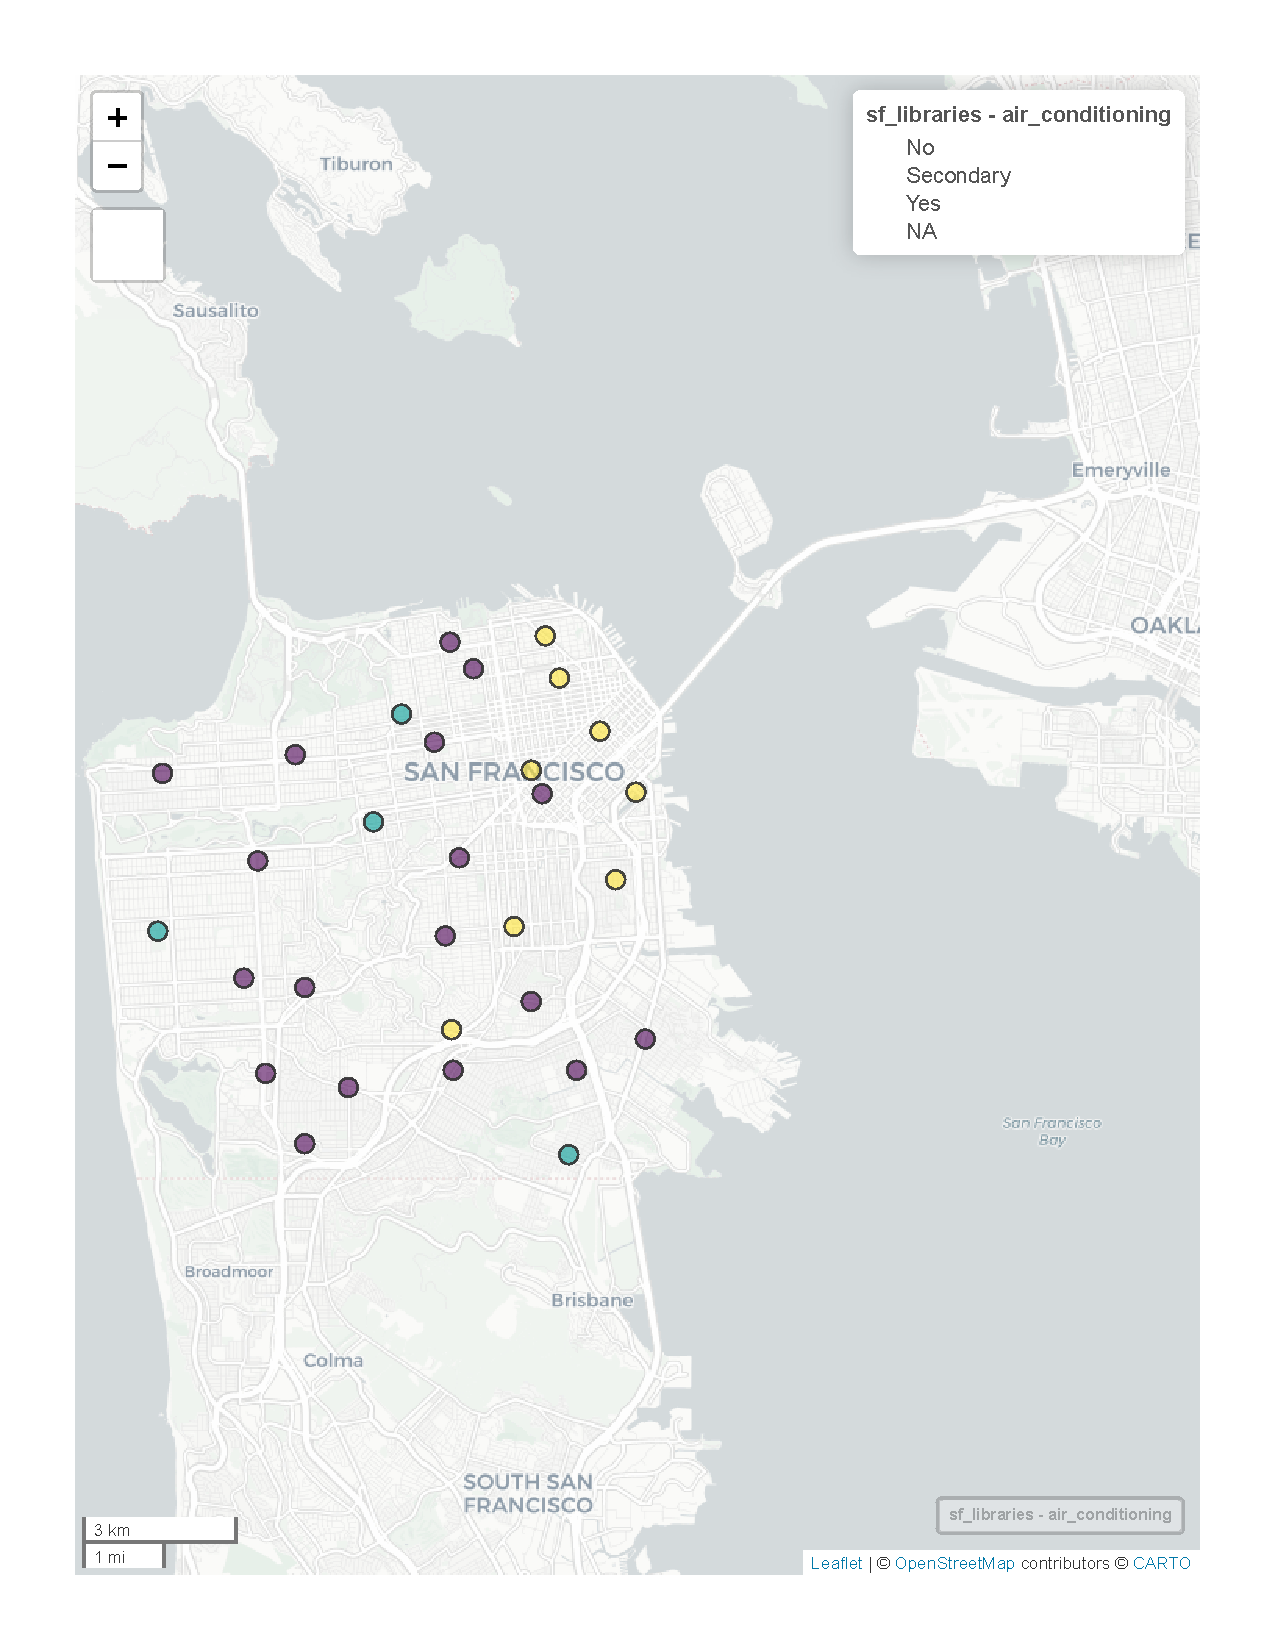
\includegraphics[keepaspectratio]{spatial_files/figure-pdf/unnamed-chunk-2-1.pdf}}

It is also convenient to wrap this up into the body of a single
function:

\begin{Shaded}
\begin{Highlighting}[]
\NormalTok{get\_arcgis\_layer }\OtherTok{\textless{}{-}} \ControlFlowTok{function}\NormalTok{(lyr\_name) \{}
\NormalTok{  url }\OtherTok{\textless{}{-}}\NormalTok{ glue}\SpecialCharTok{::}\FunctionTok{glue}\NormalTok{(}\StringTok{"https://services.arcgis.com/Zs2aNLFN00jrS4gG/arcgis/rest/services/\{lyr\_name\}/FeatureServer/0"}\NormalTok{)}
\NormalTok{  out }\OtherTok{\textless{}{-}}\NormalTok{ arcgislayers}\SpecialCharTok{::}\FunctionTok{arc\_select}\NormalTok{(arcgislayers}\SpecialCharTok{::}\FunctionTok{arc\_open}\NormalTok{(url))}
  \FunctionTok{return}\NormalTok{(out)}
\NormalTok{\}}

\NormalTok{libraries }\OtherTok{\textless{}{-}} \FunctionTok{get\_arcgis\_layer}\NormalTok{(}\StringTok{"SF\_Libraries"}\NormalTok{)}
\end{Highlighting}
\end{Shaded}

\subsection{Writing Layers}\label{writing-layers}

If you have an sfgov.maps.arcgis.com account, you can write layers
directly to your content. Read
\href{https://r.esri.com/r-bridge-site/location-services/connecting-to-a-portal.html}{the
authorization page} for more information on credentials and tokens.

\begin{Shaded}
\begin{Highlighting}[]
\NormalTok{nc }\OtherTok{\textless{}{-}} \FunctionTok{st\_read}\NormalTok{(}\FunctionTok{system.file}\NormalTok{(}\StringTok{"shape/nc.shp"}\NormalTok{, }\AttributeTok{package =} \StringTok{"sf"}\NormalTok{))}
\NormalTok{tkn }\OtherTok{\textless{}{-}} \FunctionTok{auth\_code}\NormalTok{()}
\FunctionTok{set\_arc\_token}\NormalTok{(tkn)}

\NormalTok{publish\_res }\OtherTok{\textless{}{-}} \FunctionTok{publish\_layer}\NormalTok{(nc, }\StringTok{"North Carolina SIDS sample"}\NormalTok{)}
\end{Highlighting}
\end{Shaded}

\section{ArcGIS Pro}\label{arcgis-pro}

If you have an ArcGIS Pro license, you can write directly to
geodatabases within Projects using the \{arcgisbinding\} package.

\begin{verbatim}
Reading layer `OGRGeoJSON' from data source 
  `https://data.sfgov.org/api/geospatial/f2zs-jevy?accessType=DOWNLOAD&method=export&format=GeoJSON' 
  using driver `GeoJSON'
Simple feature collection with 11 features and 7 fields
Geometry type: MULTIPOLYGON
Dimension:     XY
Bounding box:  xmin: -123.1738 ymin: 37.63983 xmax: -122.3279 ymax: 37.8632
Geodetic CRS:  WGS 84
\end{verbatim}

\begin{Shaded}
\begin{Highlighting}[]
\FunctionTok{library}\NormalTok{(arcgisbinding)}
\CommentTok{\# arc.check\_product()}

\CommentTok{\# Get Supervisor Districts from DataSF:}
\NormalTok{sup\_dists }\OtherTok{\textless{}{-}} \FunctionTok{st\_read}\NormalTok{(}\StringTok{"https://data.sfgov.org/api/geospatial/f2zs{-}jevy?accessType=DOWNLOAD\&method=export\&format=GeoJSON"}\NormalTok{)}

\CommentTok{\# Write to ArcGIS Pro project geodatabase}
\NormalTok{proj\_path }\OtherTok{\textless{}{-}} \StringTok{"...\textless{}full\_path\textgreater{}.../ArcGIS/Projects/Test R Project/Test R Project.gdb/sup\_dist"}
\FunctionTok{arc.write}\NormalTok{(}\AttributeTok{path =}\NormalTok{ proj\_path, }\AttributeTok{data =}\NormalTok{ sup\_dists)}
\end{Highlighting}
\end{Shaded}

\begin{center}
\pandocbounded{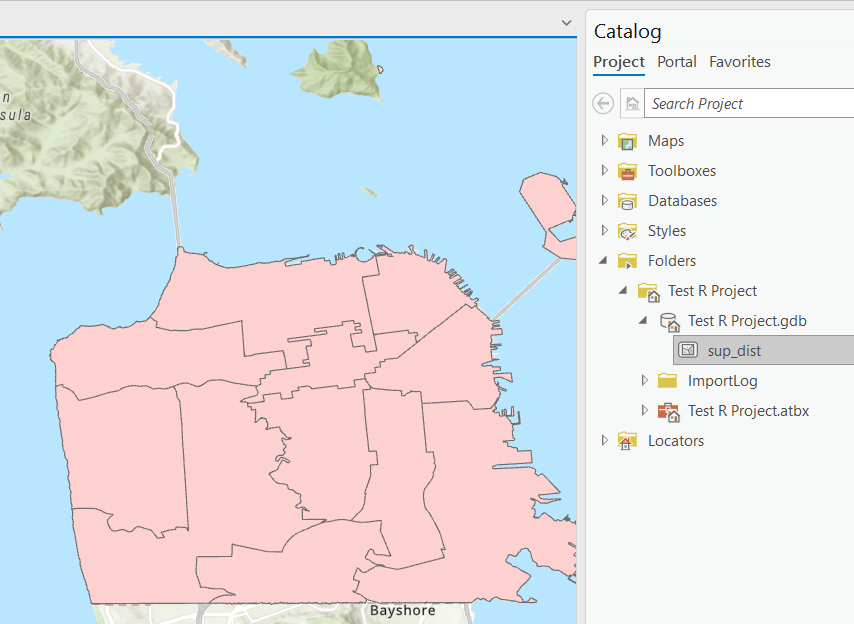
\includegraphics[keepaspectratio]{assets/arcgisbinding.png}}
\end{center}

\section{Spatial Joins}\label{spatial-joins}

Use spatial joins to determine which points are `within' which polygon:

\begin{Shaded}
\begin{Highlighting}[]
\NormalTok{nhoods }\OtherTok{\textless{}{-}} \FunctionTok{st\_read}\NormalTok{(}\StringTok{"https://data.sfgov.org/resource/j2bu{-}swwd.geojson"}\NormalTok{)}
\end{Highlighting}
\end{Shaded}

\begin{verbatim}
Reading layer `j2bu-swwd' from data source 
  `https://data.sfgov.org/resource/j2bu-swwd.geojson' using driver `GeoJSON'
Simple feature collection with 41 features and 1 field
Geometry type: MULTIPOLYGON
Dimension:     XY
Bounding box:  xmin: -122.5149 ymin: 37.70813 xmax: -122.357 ymax: 37.8333
Geodetic CRS:  WGS 84
\end{verbatim}

\begin{Shaded}
\begin{Highlighting}[]
\CommentTok{\# The coordinate reference systems must match}
\FunctionTok{st\_crs}\NormalTok{(sf\_libraries) }\SpecialCharTok{==} \FunctionTok{st\_crs}\NormalTok{(sup\_dists)}
\end{Highlighting}
\end{Shaded}

\begin{verbatim}
[1] FALSE
\end{verbatim}

\begin{Shaded}
\begin{Highlighting}[]
\NormalTok{sf\_libraries }\SpecialCharTok{\%\textgreater{}\%} 
  \FunctionTok{select}\NormalTok{(common\_nam) }\SpecialCharTok{\%\textgreater{}\%} 
  \FunctionTok{st\_transform}\NormalTok{(}\FunctionTok{st\_crs}\NormalTok{(sup\_dists)) }\SpecialCharTok{\%\textgreater{}\%} 
  \FunctionTok{st\_join}\NormalTok{(sup\_dists }\SpecialCharTok{\%\textgreater{}\%} \FunctionTok{select}\NormalTok{(sup\_dist), }\AttributeTok{join =}\NormalTok{ st\_within) }\SpecialCharTok{\%\textgreater{}\%} 
  \FunctionTok{st\_join}\NormalTok{(nhoods, }\AttributeTok{join =}\NormalTok{ st\_within) }\SpecialCharTok{\%\textgreater{}\%} 
  \FunctionTok{st\_drop\_geometry}\NormalTok{() }\SpecialCharTok{\%\textgreater{}\%} 
  \FunctionTok{mutate}\NormalTok{(}\AttributeTok{common\_nam =} \FunctionTok{gsub}\NormalTok{(}\StringTok{" Branch| Library"}\NormalTok{, }\StringTok{""}\NormalTok{, common\_nam)) }\SpecialCharTok{\%\textgreater{}\%} 
  \FunctionTok{head}\NormalTok{()}
\end{Highlighting}
\end{Shaded}

\begin{verbatim}
                           common_nam sup_dist               nhood
1                         Mission Bay        6         Mission Bay
2 Eureka Valley/ Harvey Milk Memorial        8 Castro/Upper Market
3                          Noe Valley        8          Noe Valley
4                         West Portal        7  West of Twin Peaks
5                              Marina        2              Marina
6                           Ingleside        7  West of Twin Peaks
\end{verbatim}

\section{Removing Farallon Islands from Supervisor
Districts}\label{removing-farallon-islands-from-supervisor-districts}

\begin{Shaded}
\begin{Highlighting}[]
\NormalTok{d4 }\OtherTok{\textless{}{-}}\NormalTok{ sup\_dists }\SpecialCharTok{\%\textgreater{}\%} 
  \FunctionTok{filter}\NormalTok{(sup\_dist }\SpecialCharTok{==} \DecValTok{4}\NormalTok{) }\SpecialCharTok{\%\textgreater{}\%} 
  \FunctionTok{st\_cast}\NormalTok{(}\StringTok{"POLYGON"}\NormalTok{) }\SpecialCharTok{\%\textgreater{}\%} 
  \FunctionTok{slice}\NormalTok{(}\DecValTok{1}\NormalTok{) }\SpecialCharTok{\%\textgreater{}\%} 
  \FunctionTok{st\_cast}\NormalTok{(}\StringTok{"MULTIPOLYGON"}\NormalTok{)}
\end{Highlighting}
\end{Shaded}

\begin{verbatim}
Warning in st_cast.sf(., "POLYGON"): repeating attributes for all
sub-geometries for which they may not be constant
\end{verbatim}

\begin{Shaded}
\begin{Highlighting}[]
\NormalTok{sup\_dists\_no\_farallon }\OtherTok{\textless{}{-}}\NormalTok{ sup\_dists }\SpecialCharTok{\%\textgreater{}\%} 
  \FunctionTok{filter}\NormalTok{(sup\_dist }\SpecialCharTok{!=} \DecValTok{4}\NormalTok{) }\SpecialCharTok{\%\textgreater{}\%} 
  \FunctionTok{bind\_rows}\NormalTok{(d4)}

\FunctionTok{mapview}\NormalTok{(sup\_dists\_no\_farallon)}
\end{Highlighting}
\end{Shaded}

\pandocbounded{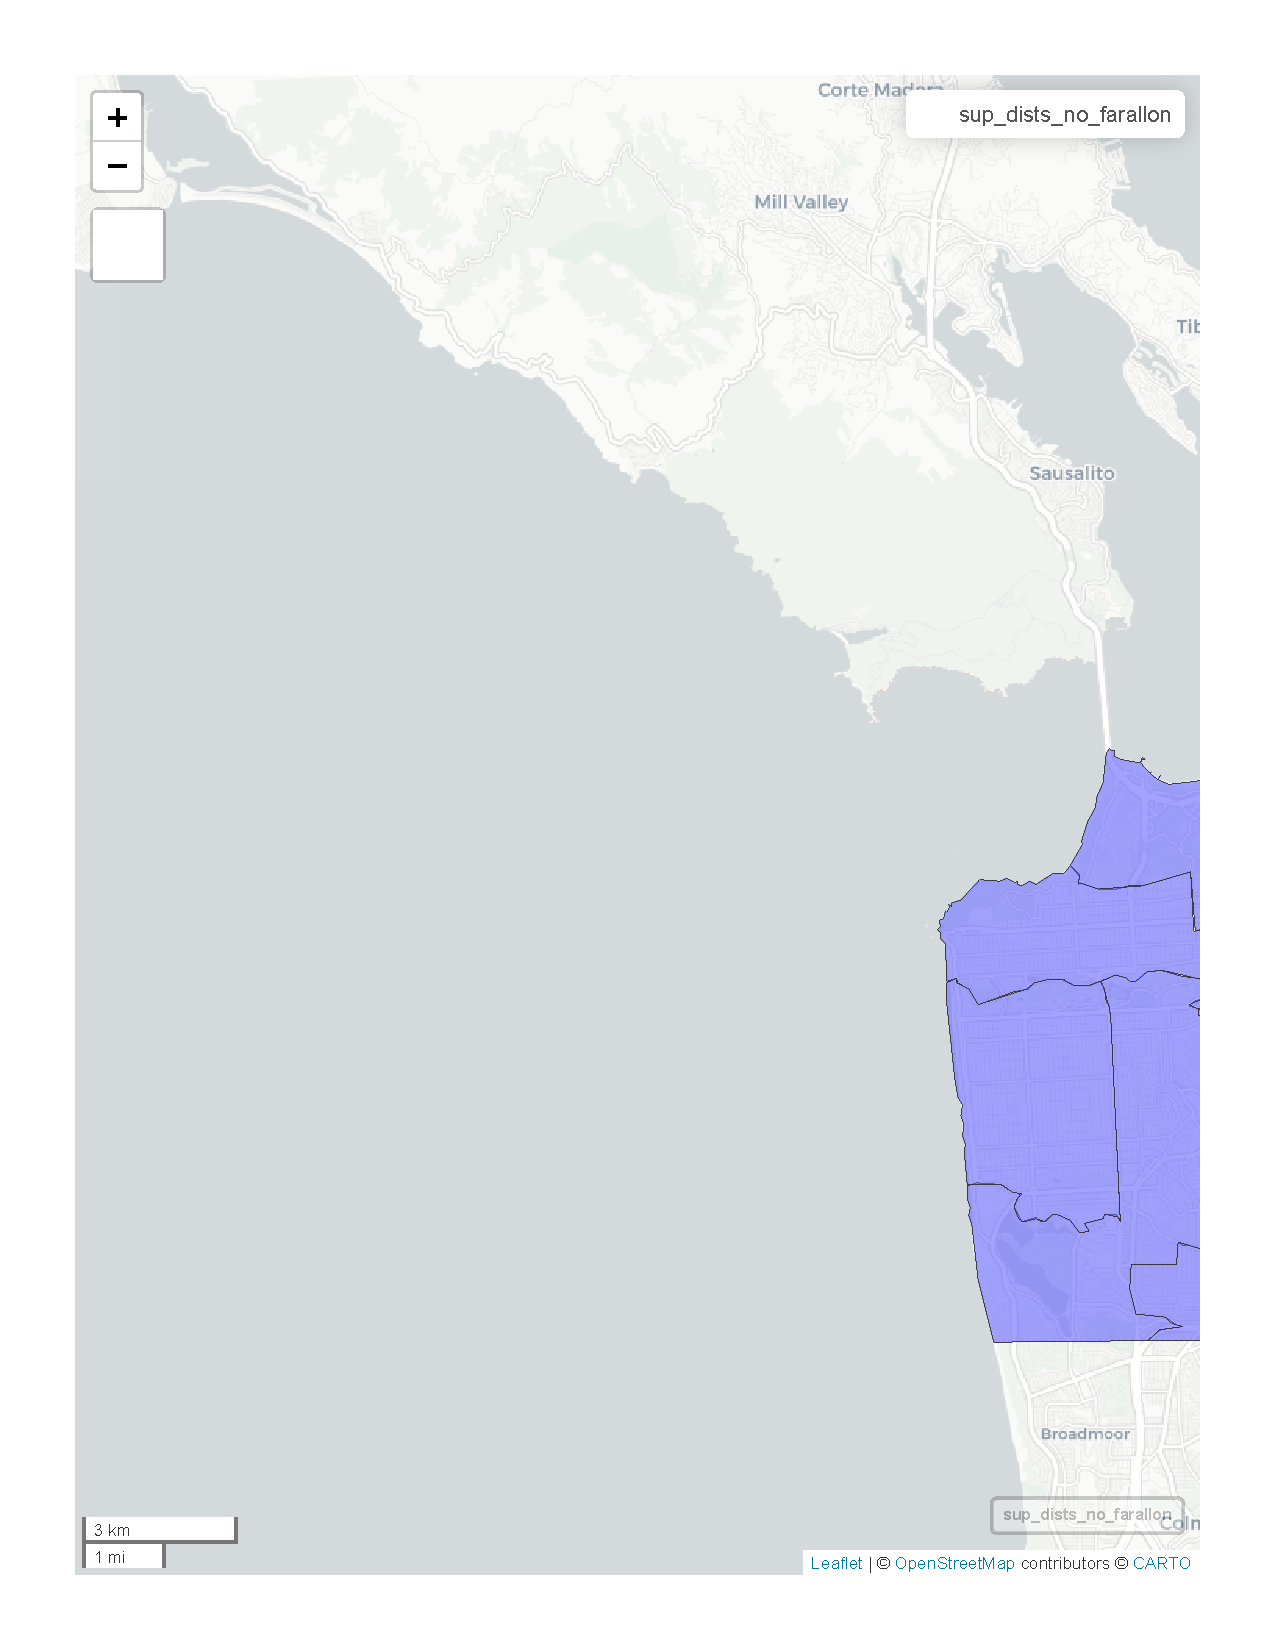
\includegraphics[keepaspectratio]{spatial_files/figure-pdf/unnamed-chunk-8-1.pdf}}

\section{Census Data}\label{census-data}

The \href{https://walker-data.com/tidycensus/}{\{tidycensus package\}}
is fantastic, and the documentation is full of helpful examples.

\begin{Shaded}
\begin{Highlighting}[]
\FunctionTok{library}\NormalTok{(tidycensus)}

\NormalTok{sf }\OtherTok{\textless{}{-}} \FunctionTok{get\_acs}\NormalTok{(}
  \AttributeTok{state =} \StringTok{"CA"}\NormalTok{,}
  \AttributeTok{county =} \StringTok{"San Francisco"}\NormalTok{,}
  \AttributeTok{geography =} \StringTok{"tract"}\NormalTok{,}
  \AttributeTok{variables =} \StringTok{"B19013\_001"}\NormalTok{,}
  \AttributeTok{geometry =} \ConstantTok{TRUE}\NormalTok{,}
  \AttributeTok{year =} \DecValTok{2020}
\NormalTok{) }\SpecialCharTok{\%\textgreater{}\%} 
  \FunctionTok{st\_transform}\NormalTok{(}\DecValTok{3857}\NormalTok{)}
\end{Highlighting}
\end{Shaded}

\begin{verbatim}
Getting data from the 2016-2020 5-year ACS
\end{verbatim}

\begin{verbatim}
Downloading feature geometry from the Census website.  To cache shapefiles for use in future sessions, set `options(tigris_use_cache = TRUE)`.
\end{verbatim}

\begin{Shaded}
\begin{Highlighting}[]
\NormalTok{sf\_bbox }\OtherTok{\textless{}{-}}\NormalTok{ libraries }\SpecialCharTok{\%\textgreater{}\%} 
  \FunctionTok{drop\_na}\NormalTok{(city) }\SpecialCharTok{\%\textgreater{}\%} 
  \FunctionTok{st\_buffer}\NormalTok{(}\DecValTok{3500}\NormalTok{) }\SpecialCharTok{\%\textgreater{}\%} 
  \FunctionTok{st\_bbox}\NormalTok{()}
  
\NormalTok{sf }\SpecialCharTok{\%\textgreater{}\%}
  \FunctionTok{ggplot}\NormalTok{(}\FunctionTok{aes}\NormalTok{(}\AttributeTok{fill =}\NormalTok{ estimate)) }\SpecialCharTok{+} 
  \FunctionTok{geom\_sf}\NormalTok{(}\AttributeTok{color =} \ConstantTok{NA}\NormalTok{) }\SpecialCharTok{+} 
  \FunctionTok{labs}\NormalTok{(}\AttributeTok{title =} \StringTok{"Median Household Income, 2020"}\NormalTok{, }\AttributeTok{fill =} \ConstantTok{NULL}\NormalTok{) }\SpecialCharTok{+}
  \FunctionTok{coord\_sf}\NormalTok{(}\AttributeTok{xlim =}\NormalTok{ sf\_bbox[}\FunctionTok{c}\NormalTok{(}\StringTok{"xmin"}\NormalTok{, }\StringTok{"xmax"}\NormalTok{)], }\AttributeTok{ylim =}\NormalTok{ sf\_bbox[}\FunctionTok{c}\NormalTok{(}\StringTok{"ymin"}\NormalTok{, }\StringTok{"ymax"}\NormalTok{)], }\AttributeTok{expand =} \ConstantTok{TRUE}\NormalTok{) }\SpecialCharTok{+}
  \FunctionTok{scale\_fill\_viridis\_c}\NormalTok{(}\AttributeTok{option =} \StringTok{"magma"}\NormalTok{, }\AttributeTok{labels =}\NormalTok{ scales}\SpecialCharTok{::}\NormalTok{dollar) }\SpecialCharTok{+}
  \FunctionTok{theme\_bw}\NormalTok{()}
\end{Highlighting}
\end{Shaded}

\pandocbounded{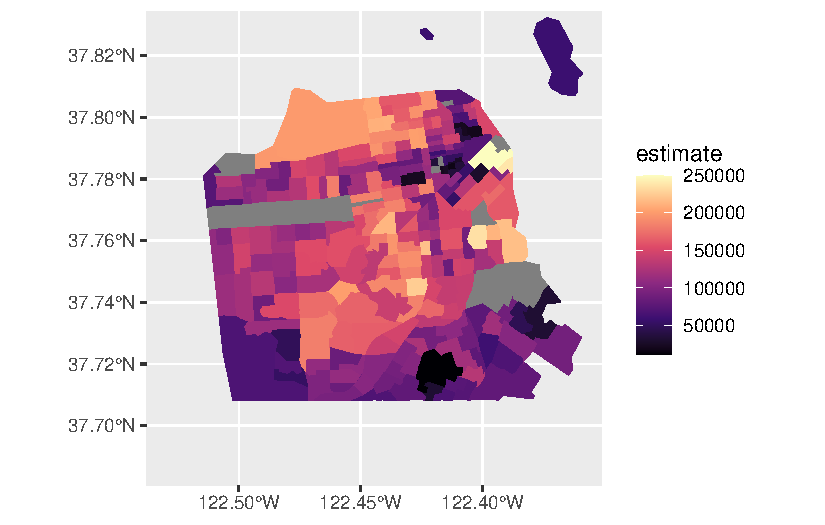
\includegraphics[keepaspectratio]{spatial_files/figure-pdf/unnamed-chunk-9-1.pdf}}

\bookmarksetup{startatroot}

\chapter{Geocoding}\label{geocoding}

\section{City Locator}\label{city-locator}

There are several ways to geocode addresses from R, but the easiest (and
cheapest) way is with the
\href{https://jessecambon.github.io/tidygeocoder/}{\{tidygeocoder\}
package} and one of the city's
\href{https://gis.sf.gov/svc/rest/services/loc/c83_eas_str_ctrl_composite/GeocodeServer/findAddressCandidates}{internal
locators.}

\begin{tcolorbox}[enhanced jigsaw, breakable, coltitle=black, opacitybacktitle=0.6, opacityback=0, leftrule=.75mm, colbacktitle=quarto-callout-note-color!10!white, toprule=.15mm, colframe=quarto-callout-note-color-frame, colback=white, left=2mm, bottomrule=.15mm, rightrule=.15mm, bottomtitle=1mm, toptitle=1mm, title=\textcolor{quarto-callout-note-color}{\faInfo}\hspace{0.5em}{Note}, titlerule=0mm, arc=.35mm]

The locator will only geocode San Francisco addresses.

\end{tcolorbox}

\begin{Shaded}
\begin{Highlighting}[]
\FunctionTok{library}\NormalTok{(tidygeocoder)}
\FunctionTok{library}\NormalTok{(sf)}
\end{Highlighting}
\end{Shaded}

\begin{verbatim}
Linking to GEOS 3.9.1, GDAL 3.4.3, PROJ 7.2.1; sf_use_s2() is TRUE
\end{verbatim}

\begin{Shaded}
\begin{Highlighting}[]
\FunctionTok{library}\NormalTok{(mapview)}
\FunctionTok{library}\NormalTok{(tidyverse)}
\end{Highlighting}
\end{Shaded}

\begin{verbatim}
-- Attaching packages --------------------------------------- tidyverse 1.3.2
--
\end{verbatim}

\begin{verbatim}
v ggplot2 3.5.1     v purrr   1.0.2
v tibble  3.2.1     v dplyr   1.1.0
v tidyr   1.2.1     v stringr 1.5.0
v readr   2.1.3     v forcats 0.5.2
-- Conflicts ------------------------------------------ tidyverse_conflicts() --
x dplyr::filter() masks stats::filter()
x dplyr::lag()    masks stats::lag()
\end{verbatim}

\begin{Shaded}
\begin{Highlighting}[]
\NormalTok{df }\OtherTok{\textless{}{-}} \FunctionTok{tibble}\NormalTok{(}\AttributeTok{address =} \FunctionTok{c}\NormalTok{(}\StringTok{"1 South Van Ness"}\NormalTok{, }\StringTok{"1 Dr Carlton B Goodlett Pl"}\NormalTok{))}
\NormalTok{locator }\OtherTok{\textless{}{-}} \StringTok{"https://gis.sf.gov/dahl/rest/services/app\_services/NRHP\_Composite/GeocodeServer/findAddressCandidates"}

\NormalTok{coords }\OtherTok{\textless{}{-}}\NormalTok{ df }\SpecialCharTok{\%\textgreater{}\%} 
  \FunctionTok{geocode}\NormalTok{(}
    \AttributeTok{api\_url =}\NormalTok{ locator,}
    \AttributeTok{address =}\NormalTok{ address,}
    \AttributeTok{custom\_query =} \FunctionTok{list}\NormalTok{(}\AttributeTok{outSR =} \StringTok{"4326"}\NormalTok{), }\CommentTok{\# outSR (Spatial Reference) is a required parameter}
    \AttributeTok{method =} \StringTok{"arcgis"}
\NormalTok{  )}
\end{Highlighting}
\end{Shaded}

\begin{verbatim}
Passing 2 addresses to the ArcGIS single address geocoder
Query completed in: 0.2 seconds
\end{verbatim}

\begin{Shaded}
\begin{Highlighting}[]
\NormalTok{coords}
\end{Highlighting}
\end{Shaded}

\begin{verbatim}
# A tibble: 2 x 3
  address                      lat  long
  <chr>                      <dbl> <dbl>
1 1 South Van Ness            37.8 -122.
2 1 Dr Carlton B Goodlett Pl  37.8 -122.
\end{verbatim}

\begin{Shaded}
\begin{Highlighting}[]
\NormalTok{coords\_sf }\OtherTok{\textless{}{-}}\NormalTok{ coords }\SpecialCharTok{\%\textgreater{}\%} \FunctionTok{st\_as\_sf}\NormalTok{(}\AttributeTok{coords =} \FunctionTok{c}\NormalTok{(}\StringTok{"long"}\NormalTok{, }\StringTok{"lat"}\NormalTok{), }\AttributeTok{crs =} \DecValTok{4326}\NormalTok{)}
\FunctionTok{mapview}\NormalTok{(coords\_sf)}
\end{Highlighting}
\end{Shaded}

\pandocbounded{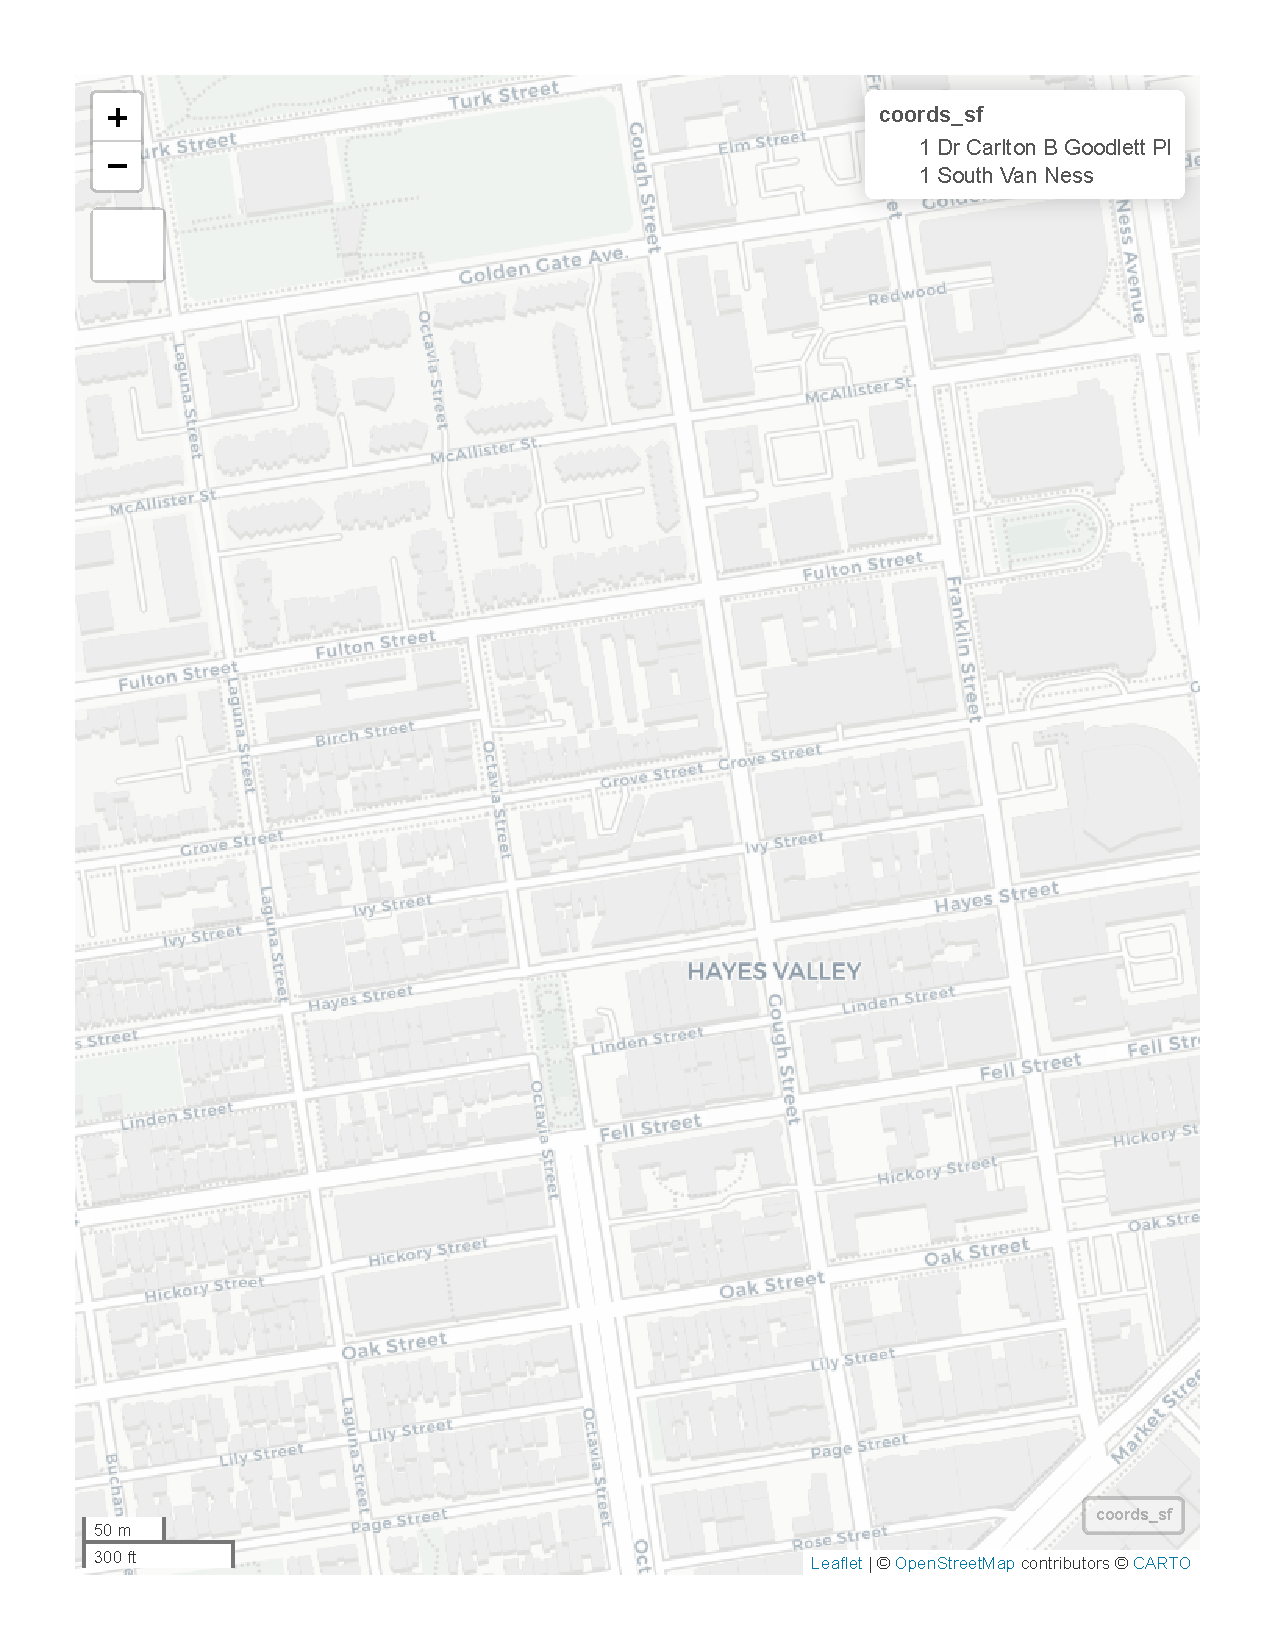
\includegraphics[keepaspectratio]{geocoding_files/figure-pdf/unnamed-chunk-1-1.pdf}}

\section{geocodio}\label{geocodio}

If you need to geocode addresses outside the city,
\href{https://www.geocod.io/}{the geocodio service} is a nice option,
but you'll first need to obtain your API key. Sign up for an account and
register for an API key. Once you have it, you need to put it in your
.Renviron file, a special text file that runs every time you
open/restart R.

Edit your .Renviron file with the usethis package:

\begin{Shaded}
\begin{Highlighting}[]
\FunctionTok{library}\NormalTok{(usethis)}
\FunctionTok{edit\_r\_environ}\NormalTok{() }\CommentTok{\# this opens the file in RStudio}
\end{Highlighting}
\end{Shaded}

Paste your API key like so:

\begin{Shaded}
\begin{Highlighting}[]
\VariableTok{GEOCODIO\_API\_KEY}\OperatorTok{=}\StringTok{\textquotesingle{}\textless{}your\_api\_key\textgreater{}\textquotesingle{}}
\end{Highlighting}
\end{Shaded}

Save the file and restart R. You should then be able to call
\texttt{geocode} with the
\texttt{method\ =\ \textquotesingle{}geocodio\textquotesingle{}}
argument. Note that there is a rate limit of 1000 addresses per hour.

\bookmarksetup{startatroot}

\chapter{Icons}\label{icons}

The Digital Services team has provided
\href{https://design-system.sf.gov/components/icons/}{a nifty set of
icons on the San Francisco Design System website.} You can use these
icons in Quarto (HTML) documents by installing
\href{https://github.com/SFOEWD/sficons?tab=readme-ov-file}{the sficons
extension from GitHub here.}

\begin{Shaded}
\begin{Highlighting}[]
\ExtensionTok{quarto}\NormalTok{ install extension SFOEWD/sficons}
\end{Highlighting}
\end{Shaded}

To embed an icon, use the \texttt{} shortcode. Some examples:

\begin{Shaded}
\begin{Highlighting}[]
\NormalTok{\{\{}\SpecialCharTok{\textless{}}\NormalTok{ sficon wip }\SpecialCharTok{\textgreater{}}\NormalTok{\}\}}
\NormalTok{\{\{}\SpecialCharTok{\textless{}}\NormalTok{ sficon alert }\SpecialCharTok{\textgreater{}}\NormalTok{\}\}}
\end{Highlighting}
\end{Shaded}

\begin{Shaded}
\begin{Highlighting}[]
\NormalTok{\{\{}\SpecialCharTok{\textless{}}\NormalTok{ sficon arrow}\SpecialCharTok{{-}}\NormalTok{right color}\OtherTok{=}\NormalTok{firebrick }\SpecialCharTok{\textgreater{}}\NormalTok{\}\}}

\NormalTok{\{\{}\SpecialCharTok{\textless{}}\NormalTok{ sficon globe color}\OtherTok{=}\NormalTok{green size}\OtherTok{=}\DecValTok{5}\NormalTok{em }\SpecialCharTok{\textgreater{}}\NormalTok{\}\}}

\NormalTok{\{\{}\SpecialCharTok{\textless{}}\NormalTok{ sficon pencil color}\OtherTok{=}\NormalTok{gold size}\OtherTok{=}\DecValTok{10}\NormalTok{em }\SpecialCharTok{\textgreater{}}\NormalTok{\}\}}
\end{Highlighting}
\end{Shaded}

Control the color and size of the icons:

\bookmarksetup{startatroot}

\chapter{Snowflake}\label{snowflake}

WIP

\section{Setup}\label{setup}

You will first need to
\href{https://docs.snowflake.com/en/developer-guide/odbc/odbc}{install
Snowflake's ODBC Driver.} Then configure the DSN for either Windows or
macOS.

\section{Making the Connection}\label{making-the-connection}

I wrapped the connection into a function:

\begin{Shaded}
\begin{Highlighting}[]
\NormalTok{connect\_to\_snowflake }\OtherTok{\textless{}{-}} \ControlFlowTok{function}\NormalTok{() \{}
\NormalTok{  conn }\OtherTok{\textless{}{-}}\NormalTok{ DBI}\SpecialCharTok{::}\FunctionTok{dbConnect}\NormalTok{(}
\NormalTok{    odbc}\SpecialCharTok{::}\FunctionTok{odbc}\NormalTok{(), }
    \StringTok{"\textless{}data\_source\_name\textgreater{}"}\NormalTok{, }
    \AttributeTok{uid =} \StringTok{"\textless{}user\_id\textgreater{}"}\NormalTok{, }
    \AttributeTok{pwd =}\NormalTok{ rstudioapi}\SpecialCharTok{::}\FunctionTok{askForPassword}\NormalTok{())}
  \FunctionTok{return}\NormalTok{(conn)}
\NormalTok{\}}

\NormalTok{con }\OtherTok{\textless{}{-}} \FunctionTok{connect\_to\_snowflake}\NormalTok{()}
\end{Highlighting}
\end{Shaded}

This works fine for interactive analysis, but you will need to stash
your password as an environment variable for various workflows, or
perhaps \href{https://github.com/ropensci/targets}{within \{targets\}
projects. (see below)}

\section{Using SQL}\label{using-sql}

Like any other database connection, you can pass SQL queries to the
connection as a string.

\begin{tcolorbox}[enhanced jigsaw, breakable, coltitle=black, opacitybacktitle=0.6, opacityback=0, leftrule=.75mm, colbacktitle=quarto-callout-warning-color!10!white, toprule=.15mm, colframe=quarto-callout-warning-color-frame, colback=white, left=2mm, bottomrule=.15mm, rightrule=.15mm, bottomtitle=1mm, toptitle=1mm, title=\textcolor{quarto-callout-warning-color}{\faExclamationTriangle}\hspace{0.5em}{Warning}, titlerule=0mm, arc=.35mm]

If you set a default schema when configuring your Snowflake data source,
you must explicitly reference other schemas when querying tables outside
of it.

\end{tcolorbox}

\begin{Shaded}
\begin{Highlighting}[]
\NormalTok{DBI}\SpecialCharTok{::}\FunctionTok{dbGetQuery}\NormalTok{(}
\NormalTok{  con,}
  \StringTok{"select table\_name, last\_altered}
\StringTok{  from information\_schema.tables }
\StringTok{  where table\_name like \textquotesingle{}STG\%\textquotesingle{} limit 5}
\StringTok{  "}\NormalTok{)}
\end{Highlighting}
\end{Shaded}

\section{Using R}\label{using-r}

\begin{Shaded}
\begin{Highlighting}[]
\NormalTok{is }\OtherTok{\textless{}{-}} \FunctionTok{tbl}\NormalTok{(con, }\FunctionTok{in\_schema}\NormalTok{(}\StringTok{"INFORMATION\_SCHEMA"}\NormalTok{, }\StringTok{"TABLES"}\NormalTok{))}
\NormalTok{is }\SpecialCharTok{\%\textgreater{}\%} 
  \FunctionTok{select}\NormalTok{(TABLE\_NAME, LAST\_ALTERED) }\SpecialCharTok{\%\textgreater{}\%} 
  \FunctionTok{filter}\NormalTok{(}\FunctionTok{str\_detect}\NormalTok{(TABLE\_NAME, }\StringTok{\textquotesingle{}\^{}STG\textquotesingle{}}\NormalTok{)) }\SpecialCharTok{\%\textgreater{}\%}
  \FunctionTok{head}\NormalTok{(}\DecValTok{5}\NormalTok{) }\SpecialCharTok{\%\textgreater{}\%} 
  \FunctionTok{collect}\NormalTok{()}
\end{Highlighting}
\end{Shaded}

\section{Snowflake tables as targets}\label{snowflake-tables-as-targets}

We can use \texttt{tarchetypes::tar\_change()} and the
\texttt{LAST\_ALTERED} field referenced above as a trigger in
\{targets\} pipelines. If the date changes, the target will rerun
alongside with downstream targets. Here's a small example of how that
might work:

\texttt{\_targets.R}

\begin{Shaded}
\begin{Highlighting}[]
\FunctionTok{library}\NormalTok{(targets)}
\FunctionTok{library}\NormalTok{(tarchetypes)}

\FunctionTok{tar\_option\_set}\NormalTok{(}
  \AttributeTok{packages =} \FunctionTok{c}\NormalTok{(}
    \StringTok{"tibble"}\NormalTok{,}
    \StringTok{"DBI"}\NormalTok{,}
    \StringTok{"odbc"}\NormalTok{,}
    \StringTok{"dplyr"}\NormalTok{,}
    \StringTok{"dbplyr"}
\NormalTok{    )}
\NormalTok{  )}

\NormalTok{connect\_to\_snowflake }\OtherTok{\textless{}{-}} \ControlFlowTok{function}\NormalTok{() \{}
\NormalTok{  conn }\OtherTok{\textless{}{-}}\NormalTok{ DBI}\SpecialCharTok{::}\FunctionTok{dbConnect}\NormalTok{(}
\NormalTok{    odbc}\SpecialCharTok{::}\FunctionTok{odbc}\NormalTok{(),}
    \StringTok{"\textless{}dsn\_name\textgreater{}"}\NormalTok{,}
    \AttributeTok{uid =} \StringTok{"\textless{}user\_id"}\NormalTok{,}
    \AttributeTok{pwd =} \StringTok{"\textless{}password\textgreater{}"}\NormalTok{)}
  \FunctionTok{return}\NormalTok{(conn)}
\NormalTok{\}}

\FunctionTok{tar\_plan}\NormalTok{(}
  \AttributeTok{snowflake\_con =} \FunctionTok{connect\_to\_snowflake}\NormalTok{(),}
  \FunctionTok{tar\_change}\NormalTok{(}
\NormalTok{    my\_table,}
    \FunctionTok{collect}\NormalTok{(}\FunctionTok{tbl}\NormalTok{(snowflake\_con, }\StringTok{"MY\_TABLE"}\NormalTok{)),}
    \AttributeTok{change =} \FunctionTok{dbGetQuery}\NormalTok{(}
\NormalTok{      snowflake\_con,}
      \StringTok{"select last\_altered from db.information\_schema.tables where table\_name = \textquotesingle{}MY\_TABLE\textquotesingle{} and table\_schema = \textquotesingle{}PROD\textquotesingle{}"}
\NormalTok{      )}
\NormalTok{  ),}
  \AttributeTok{my\_table\_transformed =} \FunctionTok{head}\NormalTok{(my\_table)}
\NormalTok{)}
\end{Highlighting}
\end{Shaded}

\bookmarksetup{startatroot}

\chapter{\{targets\} Pipelines}\label{targets-pipelines}

WIP

\bookmarksetup{startatroot}

\chapter*{References}\label{references}
\addcontentsline{toc}{chapter}{References}

\markboth{References}{References}

\phantomsection\label{refs}
\begin{CSLReferences}{0}{1}
\end{CSLReferences}




\end{document}
